%----------------------------------------------------------------------------------------
%    PACKAGES AND THEMES
%----------------------------------------------------------------------------------------
\documentclass[aspectratio=169,xcolor=dvipsnames]{beamer}
\makeatletter
\def\input@path{{theme/}}
\makeatother
\usetheme{CleanEasy}
\usepackage[utf8]{inputenc}
\usepackage{lmodern}
\usepackage[T1]{fontenc}
% \usepackage[brazil]{babel}
\usepackage{fix-cm}
\usepackage{amsmath}
\usepackage{mathtools}
\usepackage{listings}
\usepackage{xcolor}
\usepackage{hyperref}
\hypersetup{
    colorlinks=true,
    linkcolor=blue,
    filecolor=magenta,      
    urlcolor=cyan,
    pdftitle={Overleaf Example},
    pdfpagemode=FullScreen,
    }
\usepackage{graphicx} % Allows including images
\usepackage{booktabs} % Allows the use of \toprule, \midrule and \bottomrule in tables
\usepackage{tikz}
\usetikzlibrary{positioning, shapes, arrows, calc, decorations.pathreplacing, arrows.meta, backgrounds, patterns, overlay-beamer-styles}
\usepackage{etoolbox}
\usepackage{animate}

%----------------------------------------------------------------------------------------
%    LAYOUT CONFIGURATION
%----------------------------------------------------------------------------------------
\input{configs/configs}
%----------------------------------------------------------------------------------------
%    TITLE PAGE
%----------------------------------------------------------------------------------------
\input{configs/title_page}
%----------------------------------------------------------------------------------------


\begin{document}

\begin{frame}[plain]
  \titlepage
\end{frame}

\begin{frame}[plain]{Contents}
  \tableofcontents
\end{frame}

\section{Introducción}

\begin{frame}{Predicción versus estimación}

Considere el siguiente modelo de regresión

\begin{equation*}
    Y=\beta_XX+\beta_W W+\epsilon
\end{equation*}

Al estimar obtenemos $\hat\beta_X$ y $\hat\beta_W$, así como $se(\hat\beta_X)$ y $se(\hat\beta_W)$. Supongamos que los $se(\cdot)$ son tales que los coeficientes no son significativos ¿Quiere decir esto que las variables $X$ y $W$ no sirven para predecir $Y$?

\end{frame}

\begin{frame}

\begin{figure}
    \centering
    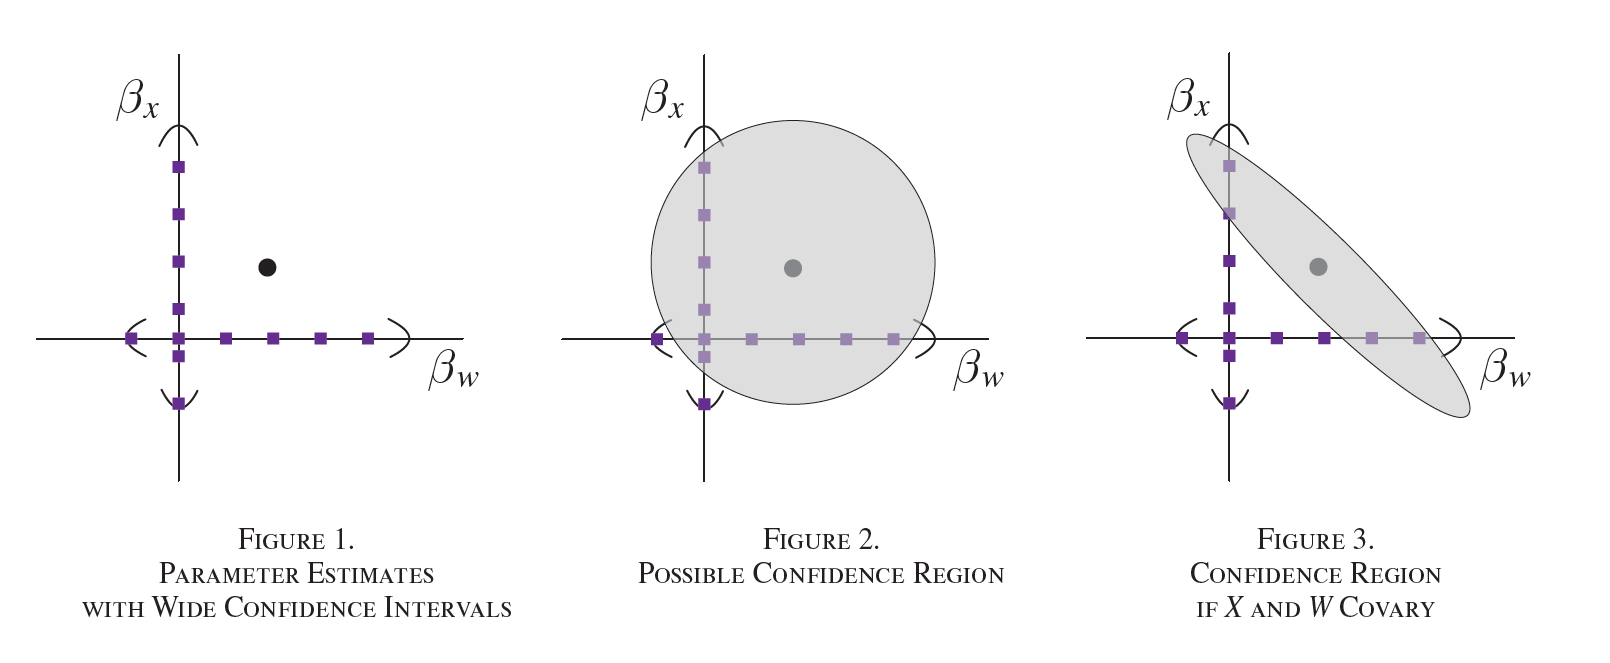
\includegraphics[width=0.8\linewidth]{fig1-3_algorithms.png}
   \end{figure}
    \end{frame}

    \begin{frame}

    \begin{itemize}
        \item Predicción: nos interesa $\hat Y$ en relación a $Y$
        \item Estimación: nos interesa $\hat\beta$
    \end{itemize}

\vspace{2mm}

    La predicción es el dominio de ML. La estimación es el dominio de la econometría

    \vspace{2mm}

    \begin{itemize}
        \item ¿Cuándo un problema es de predicción y cuándo de estimación?
        \item ¿Puede el ML apoyar en problemas de estimación? Si
    \end{itemize}
        
    \end{frame}

      \begin{frame}{Predicción vs causalidad}
        Considere los siguientes ejemplos, \cite{kleinberg2015prediction}
        \begin{itemize}
            \item Ante la amenaza de una sequía se debe decidir si se invierte en un baile para la lluvia a fin de aumentar la probabilidad de lluvia
            \item Al observar nubes en el cielo debe decidir si lleva la sombrilla para no mojarse en el camino al trabajo
        \end{itemize}

        ¿Cuál es un problema de predicción y cuál de causalidad?
    \end{frame}

    \begin{frame}{Predicción y causalidad}

    Sea $Y$ una variable de resultado que depende de una manera desconocida de la variable $X_0$. El tomador de decisión debe decidir sobre $X_0$ con el propósito de maximizar una función de pago $\pi(X_0,Y)$. La decisión depende de

    \begin{equation*}
        \dfrac{d\pi(X_0,Y)}{dX_0}=\dfrac{\partial\pi}{\partial X_0}(Y)+\dfrac{\partial \pi}{\partial Y}\dfrac{\partial Y}{\partial X_0}
    \end{equation*}

    El primer término requiere predicción, el segundo causalidad
        
    \end{frame}

    \begin{frame}{Predicción y causalidad}

    \begin{itemize}
        \item Baile para la lluvia: causalidad porque no tiene efecto directo en el pago $\frac{\partial \pi}{\partial X_0=}=0$
        \item Sombrilla: predicción pues estas no tienen ningún efecto sobre la lluvia $\frac{\partial Y}{\partial X_0}=0$
    \end{itemize}

    En el segundo caso, el valor de la acción depende del valor de $Y$. Requiere bajo error de predicción
        
    \end{frame}

\begin{frame}
    \cite{mullainathan2025economics} presenta los siguientes casos
    
    \begin{itemize}
    \item En una audiencia previa el juez debe decidir si el acusado debe ser privado o no de la libertad antes del juicio. Existe el riesgo de que el acusado escape o reincida si es dejado libre ¿La decisión del juez afecta la probabilidad de escape o reincidencia? 
    \item El juez debe decidir si le coloca el brazalete electrónico al acusado ¿La decisión del juez afecta la probabilidad de escape o reincidencia?
\end{itemize}
   
\end{frame}

\begin{frame}

\begin{figure}
    \centering
    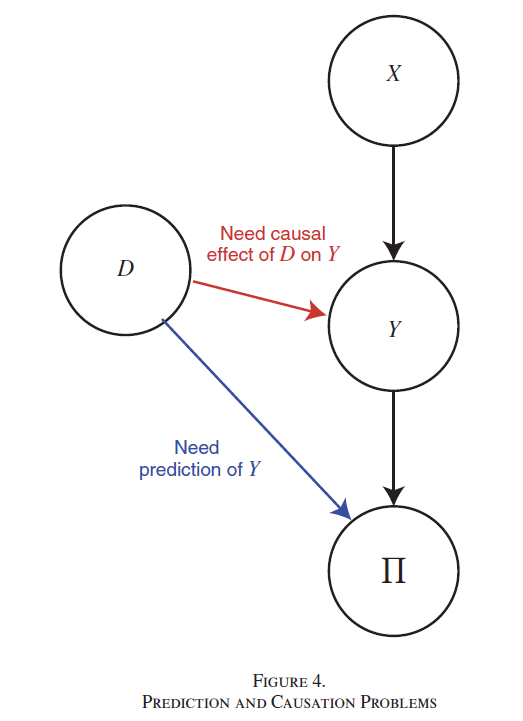
\includegraphics[width=0.4\linewidth]{fig4_algorithm.png}
    \end{figure}
    
\end{frame}

\begin{frame}{Bias variance}

    Tenemos un conjunto de datos $D$ con $n$ observaciones $(y_i,x_i)\sim G$. Usamos esta data para escoger una función $\hat{f}\in F$ para predecir $y$ con un nuevo conjunto de datos, tal que se minimice una función de pérdida, MSE (Mean Squared Error). Veamos, para un nuevo punto $x$

    \begin{equation*}
        MSE(x)=E_D[(\hat{f}(x)-y)^2]
    \end{equation*}
    Es decir, la media de la diferencia al cuadrado entre el valor predicho de $y$, $\hat{y}=\hat{f}(x)$ dado ese nuevo valor de $x$ y el valor observado/realizado de $y$
        
    \end{frame}

    \begin{frame}{Bias variance}

    Si $y=f(x)+\epsilon$, donde $\epsilon\sim (0,\sigma^2)$, entonces podemos hacer

    \begin{equation*}
        MSE(x)=E_D[(\hat{f}(x)-(f(x)+\epsilon))^2]
    \end{equation*}
        de donde se puede mostrar que
\begin{equation*}
    MSE(x)=E_D[(\hat{f}(x)-E_D(\hat{f}(x)))^2]+(E_D(\hat{f}(x))-f(x))^2+\sigma^2
\end{equation*}
El primer término recoge la varianza de la función de predicción. Que tanto varia esta de muestra a muestra. El segundo es el sesgo al cuadrado. El tercero es un error no reducible. 
    \end{frame}

    \begin{frame}{Bias variance}

    En la medida que el modelo sea más complejo, la varianza tiende a incrementarse, pero el sesgo a reducirse. 

    Si la función de predicción es MCO, 
    \begin{equation*}
    \hat{f}_{MCO}=\underset{\beta}{\mathrm{argmin}} \dfrac{1}{n}\sum_i^n (y_i-(\alpha+\beta x_i))^2  
    \end{equation*}
    
    entonces el término de bias es cero, pero la varianza es alta. MCO minimiza el error de predicción dentro de muestra, pero nos interesa el desempeño fuera de muestra
        
    \end{frame}

    \begin{frame}{Bias variance}

    Los algoritmos de ML se han diseñado para mejorar el desempeño predictivo teniendo en cuenta este bias variance trade-off. ML minimiza

    \begin{equation*}
        \hat{f}_{ML}=\underset{f\in F}{\mathrm{argmin}} \dfrac{1}{n}\sum_i^n (y_i-f(x_i))^2+\lambda R(f)  
    \end{equation*}
    donde $R(f)$ es un regularizador que penaliza las funciones que crean varianza
        
    \end{frame}

    \section{Regresión lineal predictiva}

    \begin{frame}{Regresión y el mejor predictor lineal}

    Sea $Y$ una variable escalar aleatorio y $X$ un vector de dimensión $p$ de covariables $X=(X_1,X_2,...,X_p)'$, con $X_1=1$

    \begin{itemize}
        \item Objetivo: construrir la mejor regla de predicción lineal para $Y$ usando $X$
        \item La regla será de la forma $\sum_{j=1}^p\beta_jX_j=\beta 'X$
        \item $\beta$ es cualquier solución a 
        \begin{equation*}
            \underset{b\in \mathbb{R}^p}{\mathrm{min}}E[(Y-b'X)^2]
        \end{equation*}
    \end{itemize}
        
    \end{frame}
\begin{frame}
Las C.P.O del problema anterior son

\begin{equation*}
    E[(Y-\beta'X)X]=0
\end{equation*}
La solución es el mejor predictor lineal. Si se define

\begin{equation*}
    \epsilon=(Y-\beta'X)
\end{equation*}
Entonces tenemos que la CPO es
\begin{equation*}
 E[\epsilon X]=0   
\end{equation*}
Luego el problema de mejor predicción lineal, BLP, descompone $Y$

\begin{equation*}
    Y=\beta'X+\epsilon; \quad E[\epsilon X]=0
\end{equation*}
\end{frame}
\begin{frame}{Propiedad de la mejor aproximación lineal}

La ecuación normal $ E[(Y-\beta'X)X]=0$, por ley de las expectativas iteradas
implica

\begin{equation*}
    E[(E[Y|X]-\beta 'X)X]=0
\end{equation*}
Mejor predicción lineal también es la mejor predicción lineal para la expectativa condicionada. Nos permitirá aproximar relaciones no lineales usando una especificación lineal
\end{frame}
\begin{frame}{Mejor predictor}
Sea $W$ los regresores en su forma original (raw), entonces los regresores transformados son
\begin{equation*}
X=T(W)=(T_1(W),...,T_p(W))'    
\end{equation*}
Por ejemplo

\begin{equation*}
    Y=\beta_0+\beta_1X_1+\beta_2X_2+\epsilon
\end{equation*}
donde $X_1=W_1$ y $X_2=W_1\times W_1$    
\end{frame}

\begin{frame}
    En la población, el mejor predictor de $Y$ dado $W$ es
    \begin{equation*}
        g(W)=E[Y|W]
    \end{equation*}
    La función $g(W)$ resuelve el problema de la mejor predicción
\begin{equation*}
            \underset{m(W)}{\mathrm{min}}E[(Y-m(W))^2]
        \end{equation*}

        Es decir que se minimiza el MSE entre todas las reglas de predicción. Si usamos $\beta'T(W)$ estamos aproximando a $g(W)$
    
\end{frame}
\begin{frame}
    Luego, para cualquier parámetro $b$ tenemos
    \begin{equation*}
        E[(Y-b'T(W))^2]=\underset{\text{MS Error aproximación}}{E[(g(w)-b'T(W))^2]}+\underset{\text{Constante}}{E[(Y-g(W))^2]}
    \end{equation*}
    Luego minimizar el error cuadrático medio de la predicción es lo mismo que minimizar el error cuadrático medio de la aproximación. Luego $\beta'T(W)$ es la mejor aproximación lineal al mejor predictor.

    Entre más transformaciones mejor es la aproximación
\end{frame}

\begin{frame}{Propiedades estadísticas de MCO}

Entre más transformaciones la aproximación al mejor predictor es mejor. Sin embargo, esto significa más regresores y por lo tanto parámetors a estimar. Aumenta la dimensionalidad del modelo. Problema para la estimación por mínimos cuadrados
    
\end{frame}

\begin{frame}
En la práctica observamos una muestra $\{(Y_i,X_i)\}_{i=1}^n=((Y_1,X_1),(Y_2,X_2),...,(Y_n,X_n))$

Muesta aleatoria: observaciones son realizaciones iid de la variable aleatoria (Y,X). Dado $X$, el valor predicho de $Y$ es $\sum_i^n\hat{\beta}_jX_j$, donde $\hat{\beta}$ es la solución al problema de mejor predicción lineal en la muestra

\begin{equation*}
 \underset{b\in \mathbb{R}^p}{\mathrm{min}}E_n[(Y-b'X)^2]    
\end{equation*}
Definimos los residuales como
\begin{equation*}
    \hat{\epsilon}_i=(Y_i-\hat{\beta}'X_i)
\end{equation*}
luego
\begin{equation*}
    Y_i=\hat{\beta}'X_i+\hat{\epsilon}_i; \quad E_n[X\hat{\epsilon}]=0
\end{equation*}
\end{frame}

\begin{frame}
Debemos estimar $p$ parámetros, luego necesitamos observaciones por parámetro, luego nos interesa que el ratio $p/n$ sea pequeño. Si $n$ es grande en relación a $p$, entonces la regresión lineal muestral se aproxima a la regresión lineal poblacional
    
\end{frame}

\begin{frame}{Análisis de varianza y ajuste}

En la población podemos mostrar que 

\begin{align*}
    &MSE_{pop}=E[\epsilon^2]\\
    &R^2_{pop}=\dfrac{E[(\beta'X)^2]}{E[Y^2]}=1-\dfrac{E[\epsilon^2]}{E[Y^2]}
\end{align*}
Luego en la muestra
\begin{align*}
&MSE_{s}=E_n[\hat{\epsilon}^2]\\
    &R^2_{s}=\dfrac{E_n[(\hat{\beta}'X)^2]}{E_n[Y^2]}=1-\dfrac{E[\hat{\epsilon}^2]}{E[Y^2]}    
\end{align*}
   
\end{frame}

\begin{frame}
    Cuando $p/n$ es pequeño y $n$ es grande, las medidas de ajuste de la muestra son buenas aproximaciones a las medidas poblacionales

    \begin{equation*}
        MSE_s\approx MSE_{pop}; \quad R_s^2 \approx R_{pop}^2
    \end{equation*}

    
Cuando $p/n$ no es pequeño las medidas de predicción dentro de muestra no son confiables. 

Las medidas de desempeño predictivo dentro de muestra sobreestiman el desempeño predictivo fuera de muestra

\end{frame}


\begin{frame}{Inferencia sobre efectos predictivos}

¿Cómo cambian las predicciones si el predictor cambia en una unidad mientras los demás predictores se mantienen constantes?

\vspace{2mm}

Sea $X=(D,W)'$ el vector de regresores, donde $D$ es la variable de interés

\begin{equation*}
    Y=\beta_1D+\beta_2'X+\epsilon
\end{equation*}
    $\beta_1$ indica el cambio en el valro predicho por cada unidad de cambio de $D$ ¿Cuándo puedo interpretar este coeficiente en términos causales?
\end{frame}

\begin{frame}{Partialling out}
\begin{block}{Teorema Frisch-Waugh-Lovell}
    Si tenemos las variables aleatorias $Y,D,W$ con segundo momento finito, y con $D$ que no se puede predecir perfectamente por $W$, entonces el regresor poblacional $\beta_1$ puede ser recuperado de la regresión poblacional de $\tilde{Y}$ sobre $\tilde{D}$
\end{block}
    
\end{frame}

\begin{frame}{Partialling-out}

\begin{enumerate}
    \item Regrese Y sobre W y obtenga el residual, $\tilde{Y}$
    \item Regrese D sobre W y obtenga el residual, $\tilde{D}$
    \item Regrese $\tilde{Y}$ sobre $\tilde{D}$ y obtenga $\beta_1$
\end{enumerate}

Esto funciona bien si $p/n$ es pequeño. En caso contrario, la regresión lineal muestral no es adecuada y es mejor una reducción de la dimensionalidad a través de una penalización (Lasso, Ridge,...)
    
\end{frame}

\begin{frame}{Aplicaciones\footnote{\href{https://causalml-book.org/}{Seguimos los notebooks del capítulo 1}}}
Para este ejercicio usaremos datos de mercado laboral para la ciudad de Barranquilla, Colombia, año 2024

\vspace{2mm}

\begin{enumerate}
    \item Predicción de salarios: ¿Cómo podemos usar características relevantes para predecir de mejor manera los salarios?
    \item Inferencia: ¿Cuál es la diferencia de salarios entre hombres y mujeres?
\end{enumerate}
    
\end{frame}



\begin{frame}{References}
\bibliography{reference.bib}
\bibliographystyle{apalike}
\end{frame}
\end{document}